\chapter{The AquaCrop procedure to simulate crop response to agricultural management}\label{ch:aquacrop}
\chaptermark{AquaCrop simulation procedure}

\section{Introduction}
The AquaCrop crop water productivity model AquaCrop \parencite{hsiao2009,steduto2009,raes2009,vanuytrecht2014} was developed by the Food and Agriculture Organization of the United Nations (FAO) as a tool for irrigation engineers, extension agents, agricultural policy officers and researchers, that can provide quick but accurate estimates of crop production and crop water productivity under various environmental and agronomic conditions. AquaCrop simulates daily crop canopy cover, rooting depth, transpiration, dry above-ground biomass production, yield and the soil water balance in a cropped field, based on user-specified inputs of environmental and agronomic conditions.

This chapter presents AquaCrop's input requirements and calculation procedures to simulate soil water balance and crop productivity as influenced by the environmental and agronomic conditions in the cropped field. Furthermore, this chapter intents to give a complete overview of all field management practices that can be simulated with AquaCrop as well as their effect on the standard calculation procedure. Also, evaluation and application of these field management simulation procedures is discussed. 

It should be noted that this chapter only discusses the most relevant AquaCrop calculation procedures as implemented in AquaCrop version 4.0 and 5.0. More detailed information on the algorithms and calculation procedures can be found in the AquaCrop reference manuals \parencite{raes2012,raes2015b}. 

\section{Input requirements}
AquaCrop requires few data for input and calibration. In addition, the required input is either readily available from agricultural statistics and indigenous farmer knowledge, or can be directly measured in the field with straightforward and inexpensive methods \parencite{vanuytrecht2014}. This makes the model easier and more widely applicable than other crop models such as CropSyst, CERES and WOFOST, in particular for data-scarce regions \parencite{castanedavera2015,todorovic2009,abisaab2015}.

The core input of AquaCrop is specification of the cultivated crop and its (trans)planting date. Crop characteristics are described by a set of crop parameters (\autoref{tab:AnA_croppar}), which include both conservative and non-conservative parameters. While the former do not change with time and are valid for various environmental conditions, management practices and cultivars, the later need calibration to match the local cultivar and cropping system. Non-conservative parameters include amongst others growing cycle length, length of different growing stages, plant density, maximum canopy cover, maximum rooting depth and crop response to soil fertility. Conservative parameters, on the other hand, include for example the water stress and temperature stress thresholds for crop development and biomass production. The AquaCrop database includes default sets of crop parameters for 14 crops including widely cultivated crops such as barley, maize, wheat and cotton \parencite{garciavila2009,heng2009,andarzian2011,abrha2012} as well as under-utilized crops such as quinoa and tef \parencite{geerts2009,tsegay2012}. When using these default sets, only the non-conservative parameters need to be fine-tuned to local conditions. In total, parameter sets for more than 30 crops, calibrated for local conditions, have been presented in literature. These can be used as starting values when calibrating conservative and non-conservative crop parameters for crops that are not included in the AquaCrop database. 

Besides information on crop characteristics and the (trans)planting date of the selected crop, AquaCrop requires user-specified input describing the environmental and agronomic conditions of the cropped field. 

Required weather data include precipitation, minimum and maximum temperature (\Tmin and \Tmax) and reference evapotranspiration (\ETo) calculated with the FAO penman monteith method \parencite{allen1998}. Ideally, weather data are supplied on a daily basis, but the model can interpolate between 10-daily or monthly values of \Tmin, \Tmax and \ETo as well. In addition to these weather data, also annual average atmospheric \COtwo concentration ([CO$_2$]) is a required climate input parameter.  By default, AquaCrop uses historical [CO$_2$] measurements of the Mauna Loa Observatory in Hawaii. However, [CO$_2$] can also be specified by the user for past or future years according to a certain \COtwo emission scenario.

Besides weather data, soil profile characteristics need to be defined. A soil profile can consist of up to 5 soil layers, each with its own set of parameters. These parameters include the layer thickness, saturated hydraulic conductivity (\Ksat) and the volumetric water content at saturation ($\theta_{SAT}$), field capacity ($\theta_{FC}$) and permanent wilting point ($\theta_{PWP}$). The latter two define the total available soil water content (TAW). In addition, also soil surface characteristics (curve number (CN) and readily evaporable water (REW)), the depth of a soil layer blocking root growth (if present) and parameters defining capillary rise from the groundwater table need to be specified. Soil parameters can be specified based on field measurements, or the default values based on soil texture (\autoref{tab:AnA_soilpar}) can be used.

Furthermore, the groundwater, being the lower boundary condition to the soil profile, needs to be characterized with respect to its depth below the soil surface (either constant or time variable) and quality of the water. Also, information on the applied irrigation and field management practices , both during and outside the growing season, need to be specified (see \autoref{sec:ch2_Mgmt}). Finally, the model requires specification of the simulation period as well as initial conditions of soil water and salinity content. 
 
\section{Crop canopy development and production}\label{sec:ch2_ACsteps}
Being a water-driven model, AquaCrop calculates crop production based on the amount of water transpired by the crop with a four step process. In a first step, the crop's green crop canopy cover (CC) is simulated. The expansion of the canopy cover under non-stressed conditions from its initial value (\CCo) to reach the maximum canopy cover (\CCx) is described by a logistic function determined by the canopy growth coefficient (cgc). In the late season stage, the decline of the canopy cover due to senescence is described by means of the canopy decline coefficient (cdc). In a second step, crop transpiration (\Tr) (\autoref{eq:ch2_Tr}) is simulated considering weather conditions (\ETo) and a crop transpiration coefficient ($Kc_{Tr}$) that is proportional to the simulated canopy cover. Next, crop transpiration is converted into dry above-ground biomass production (\B) by means of the normalized crop water productivity (\WPster) (\autoref{eq:ch2_B}). In a final step, crop biomass is converted to crop yield by means of the harvest index (\HI) (\autoref{eq:ch2_Y}). Crop yield per unit of water evapotranspired in the cropped field is given by the ET crop water productivity (\WPET) (\autoref{eq:ch2_WPET}). Additionally, this four step process is influenced by various abiotic factors (\autoref{sec:ch2_abioticfac}) and agricultural management practices \autoref{sec:ch2_Mgmt}). 
\begin{equation}
 Tr_{i}=Ks_{i} \cdot Kc_{Tr_{i}} \cdot ET_{0_{i}}
  \label{eq:ch2_Tr}
\end{equation}
\begin{equation}
 B=Ks_{b_{i} } \cdot wp^{*} \cdot \sum_{i=1}^n \frac{Tr_{i}}{ET_{0_{i}}}
 \label{eq:ch2_B}
\end{equation}
\begin{equation}
 Y=hi \cdot B
 \label{eq:ch2_Y}
\end{equation}
\begin{equation}
 WP_{ET}=Y\sum_{i=1}^n {ET_{i}}
 \label{eq:ch2_WPET}
\end{equation}
where $Tr_{i}$ is the crop transpiration (\si{mm/day}) on day i, $ET_{0_{i}}$ is the reference evapotranspiration (\si{mm/day}), $Kc_{Tr_{i}}$ is the crop transpiration coefficient (-) proportional to the crop’s canopy cover (\CC, \si{m^2/m^2}), $Ks_{i}$ is the soil water and soil salinity stress coefficient (-), $Ks_{b_{i}}$ is the cold stress coefficient for biomass production (-), \B is the cumulative dry above-ground biomass production ($g/m^{2}$), \WPster is the normalized crop water productivity ($g/m^{2}$), \Y is the dry mass of yield ($g/m^{2}$), \HI is the harvest index (g/g), \ET is the crop evapotranspiration, \WPET is the ET crop water productivity ($kg/m^{3}$), and n is the number of sequential days spanning the growing period.

\begin{figure}[tbhp]
	\centering
		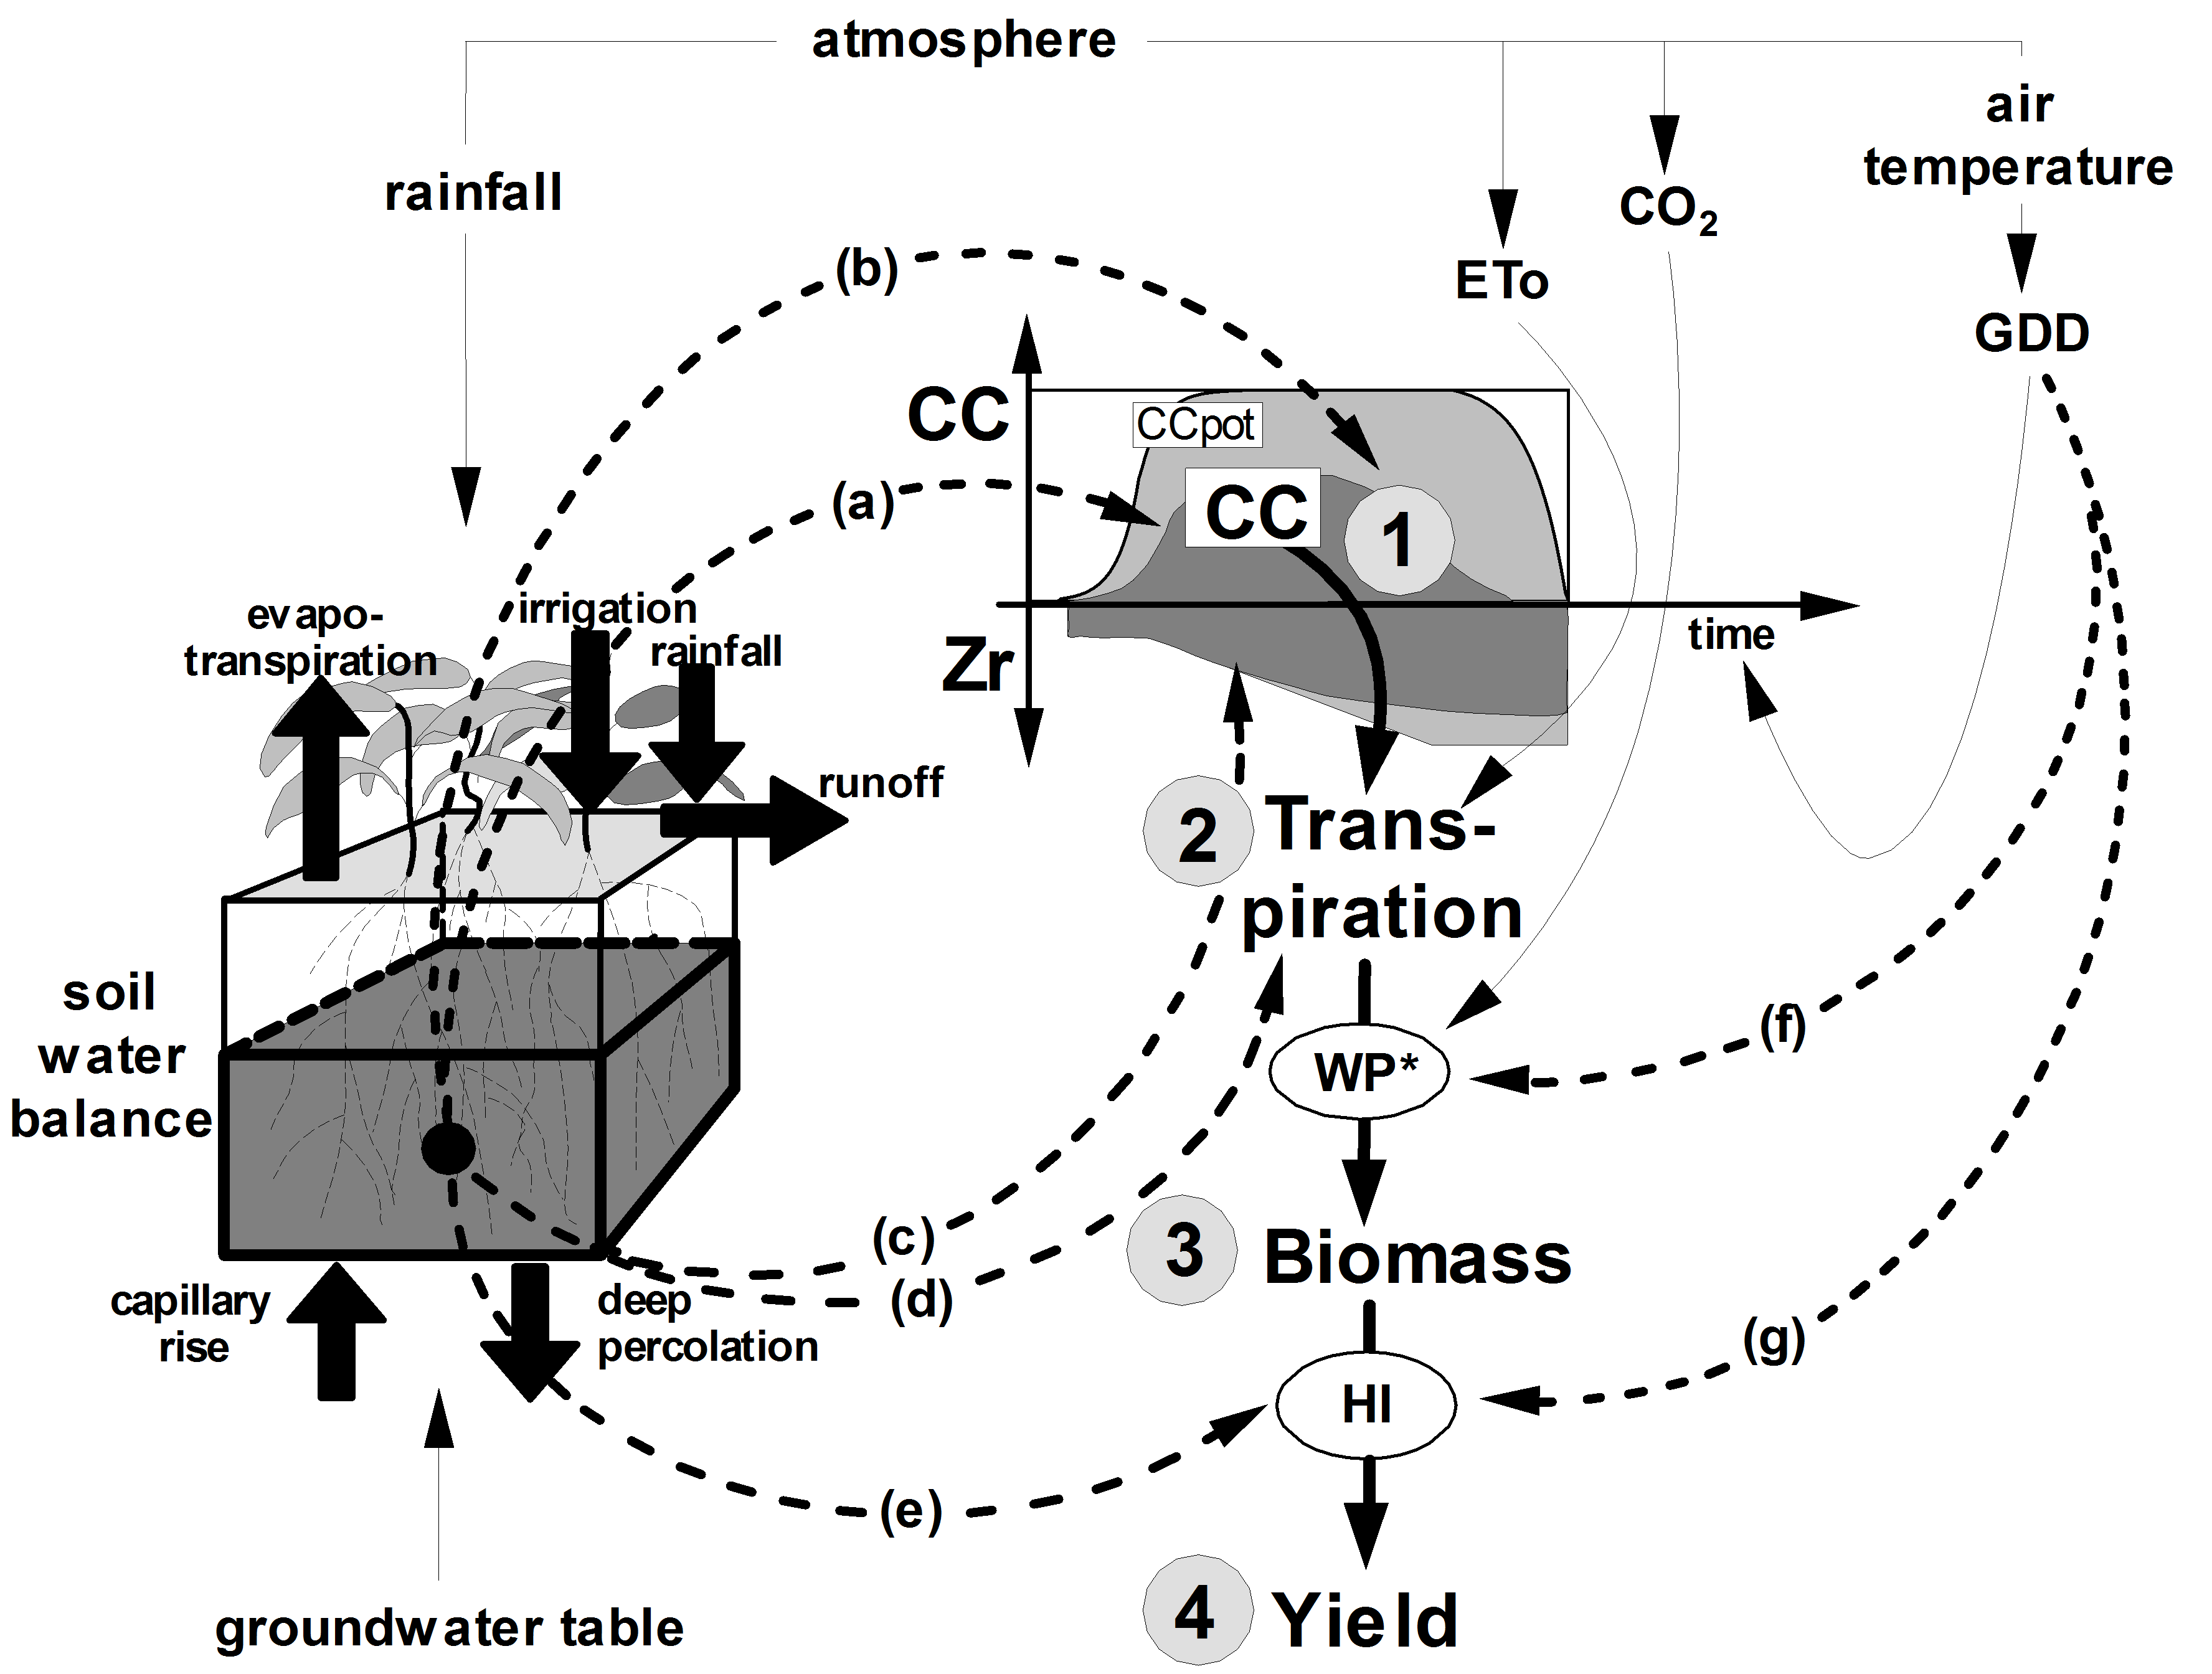
\includegraphics[width=10cm]{AC_600dpi.png}
	\caption{Calculation scheme of AquaCrop with indication of the four steps and the processess affected by water stress (dotted arrows a to e) and temperature stress (dotted arrows f to g).}
	\label{fig:ch2_AC}
\end{figure}

AquaCrop simulation results of soil water content, green canopy cover, dry above-ground biomass production and crop yield can be evaluated against field observations by means of graphical displays as well as statistical performance indicators (Box \ref{box:ch2_Eval}).

\clearpage
\newtcolorbox[auto counter,number within=chapter]{MyBox}[1][]{
  enhanced,
  unbreakable,
  %float,
  parbox=false, % zodat de paragrafen zijn zoals in de text
  title=Box \thetcbcounter : Model performance indicators,
  #1} % dit is voor het label te fixen

\begin{MyBox}[label = box:ch2_Eval]
Following statistical performance indicators will be considered in this research:

(i) the coefficient of determination or squared Pearson’s correlation coefficient (\Rsq, -): 
\begin{equation}
 R^{2}=\left(\dfrac{\sum_{i=1}^n(O_{i}-\overline{O})(P_{i}-\overline{P})}
                   {\sqrt{\sum_{i=1}^n(O_{i}-\overline{O})^2}  \cdot \sqrt{\sum_{i=1}^n(P_{i}-\overline{P})^2 }}
 \right)
  \label{eq:ch2_Rsq}
\end{equation}

(ii) the relative root-mean-square error (RRMSE,\%)\parencite{loague1991}
\begin{equation}
\begin{split}
 RRMSE&=RMSE \cdot \frac{100}{\overline{O}}\\
 &=\dfrac{\sqrt{\sum_{i=1}^n(O_{i}-P_{i})^2}}{n} \cdot \frac{100}{\overline{O}}
 \end{split}
  \label{eq:ch2_RRMSE}
\end{equation}

(iii) the Nash-Sutcliffe model efficiency (EF, -) \parencite{nash1970}:
\begin{equation}
\dfrac{\sum_{i=1}^n(P_{i}-O_{i})^2}{\sum_{i=1}^n(O_{i}-\overline{O})^2}
  \label{eq:ch2_EF}
\end{equation}

(iv) the relative model error (RME, \%) \parencite{bennett2013}:
\begin{equation}
\dfrac{\sum_{i=1}^n(O_{i}-P_{i})}{\sum_{i=1}^n(O_{i})}\cdot 100
  \label{eq:ch2_RME}
\end{equation}
where $O_{i}$ are the observed values, $P_{i}$ are the predicted values, \=O is the mean of the observed values, \=P is the mean of the predicted values and n is the number of observations.

Model performance is considered better when \Rsq and EF approach one, and when RRMSE and RME approach zero. Following \textcite{jamieson1991}, model performance can be classified based on RRMSE values as excellent (RRMSE < 10 \%), good (10 \% < RRMSE < 20 \%), fair (20 \% < RRMSE < 30 \%) and poor (RRMSE > 30 \%). 
\end{MyBox}

\section{Soil water balance}\label{sec:ch2_SWB} 
AquaCrop calculates the daily soil water content (\SWC) in the soil profile by means of a soil water balance that keeps track of incoming (rainfall, irrigation, capillary rise) and outgoing (surface runoff, deep percolation, evaporation, crop transpiration) water fluxes (\autoref{fig:ch2_SWB}). While rainfall and irrigation are user-specified inputs, other components of the soil water balance are simulated on the basis of the simulated crop canopy development as well as input of daily weather data, the depth of the groundwater table and soil characteristics.

\begin{figure}[tbhp]
	\centering
		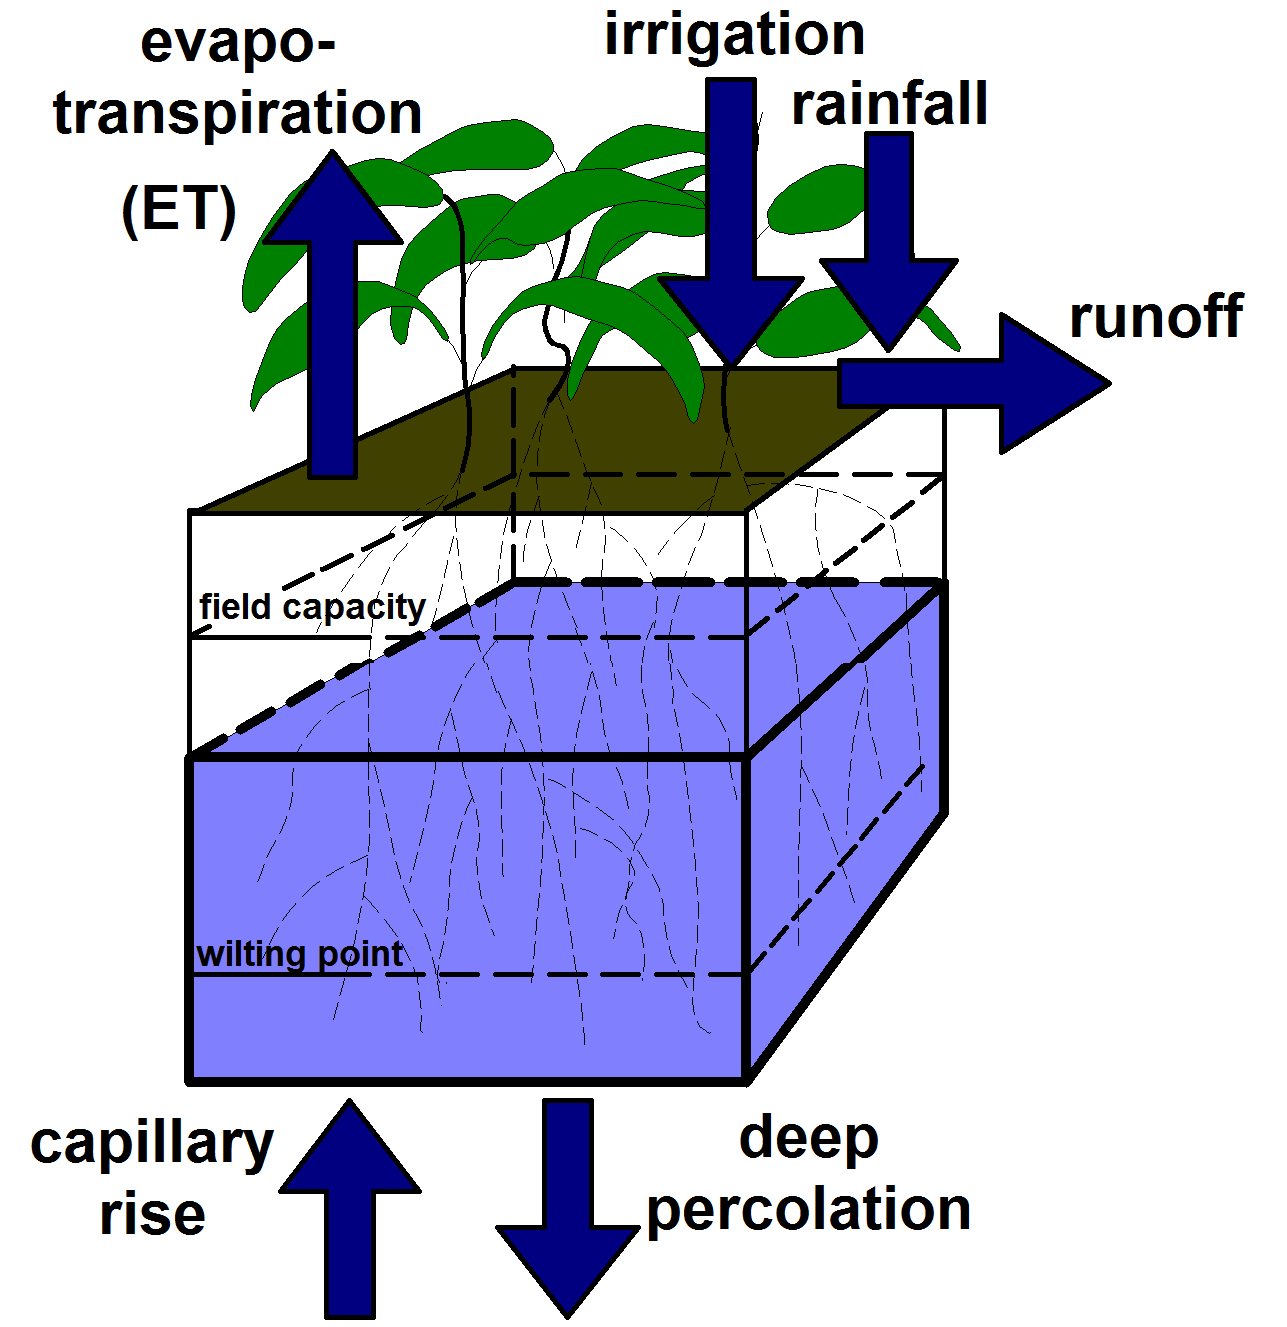
\includegraphics[]{SWB_600dpi.png}
	\caption{AquaCrop determines the soil water content in the root zone by calculating the soil water balance of incomming and outgoing water fluxes}
	\label{fig:ch2_SWB}
\end{figure}

\subsection{Crop transpiration and soil evaporation}
Crop transpiration (Tr, \autoref{eq:ch2_Tr}) and soil evaporation (\E, \autoref{eq:ch2_E}) are simulated as separate components of the soil water balance. 
\begin{equation}
 E_{i}=Kr_{i} \cdot Ke_{i} \cdot ET_{0_{i}}
  \label{eq:ch2_E}
\end{equation}
where $E_{i}$ is soil evaporation (\si{mm/day}) on day i, $Kr_{i}$ is the evaporation reduction coefficient (-), $Ke_{i}$ the evaporation coefficient (-) proportional to the non-covered soil fraction (1-\CC), and $ET_{0_{i}}$ is the reference evapotranspiration (\si{mm/day}).

Both components are proportional to the evaporative power of the atmosphere (\ETo) and simulated crop canopy cover via the crop transpiration ($Kc_{Tr}$) and evaporation (Ke) coefficients, respectively (\autoref{eq:ch2_Tr} and \ref{eq:ch2_E}). In addition, transpiration and evaporation are adjusted to the soil water content and corresponding water stress which is expressed indirectly by the CC and directly by the soil water stress (Ks) or evaporation reduction (Kr) coefficient. 

\subsection{Surface runoff}\label{sec:ch2_RO} 
Surface runoff ($RO$) is calculated using the \textcite{usda1969} curve number (CN) equation:
\begin{equation}
    RO_{i}= 
	\begin{cases}
    0 &\text{if } P_{i} \leq I_a\\
    \dfrac{(P_{i}-I_a)^2}{P_{i}-I_a+S)}&\text{if } P_{i}>I_a
	\end{cases}
\label{eq:ch2_RO}
\end{equation}
where $RO_{i}$ is surface runoff (\si{mm/day}) on day i, $P_{i}$ is rainfall (\si{mm/day}), $I_a$ initial abstraction (\si{mm}) and S is storage capacity (\si{mm}). Surface storage is derived from the runoff curve number (CN) with equation:  
  \begin{equation}
 S=254 \cdot \frac{CN}{100}-1
\label{eq:ch2_CN}
 \end{equation}
where $CN$ is the runoff curve number (-) equal to the CN value selected by the user on the basis of soil and field management characteristics (CN$_{input}$), but automatically adjusted to soil moisture conditions during simulation.
  \begin{equation}
 CN=CN_{input} \cdot f_{CN,SWC}
\label{eq:ch2_CNswc}
 \end{equation}
where $CN_{input}$ is the user-specified curve number (-) and $f_{CN,SWC}$ the correction factor for the soil water content in the top soil (by default set to a thickness of 0.3 m).

In the framework of this PhD research, the surface runoff calculation procedures have been revised in according to latest advances on the curve number approach \parencite{hawkins2009}. The revised procedures as implemented in AquaCrop version 5.0 contain two major changes. First, the standard value of initial abstraction has been altered. Originally, AquaCrop applied the common assumption that $I_a$ equals 20\% of the storage capacity. However, it was found that 5\% of S is a more appropriate value for general application \parencite{hawkins2009}. Consequently, this value was adopted as the new standard in AquaCrop version 5.0. It should be noted that also the $CN$ input values should correspond to this assumption. Hence, CN values for $I_a=20\%S$, such as found in the SCS curve number tables \parencite{usda2007}, should be converted before they are used as AquaCrop input. This can be done by means of the conversion equation proposed by \textcite{jiang2001}. %\parencite[cited in][]{hawkins2009}.

A second update was inspired by the fact that surface runoff depends as much on soil properties as on field surface management. Therefore, $CN_{input}$ is no longer uniquely defined based on soil properties (\Ksat). In AquaCrop version 5.0 the $CN$ specified as soil parameter (by default linked to the topsoil \Ksat) is adjusted for field surface management (see \autoref{sec:ch2_SurfMan}).
  \begin{equation}
 CN_{input}=CN_{soil}\cdot f_{CN,mgmt}
\label{eq:ch2_CNmgmt}
 \end{equation}
where $CN_{soil}$ is the input curve number as defined by soil properties (-) and $f_{CN,mgmt}$ is the adjustment factor for field surface management.

\subsection{Deep percolation and capillary rise}
To simulate vertical movement of water, the soil profile is divided into soil compartments of 10 cm by default. When the soil water content in one compartment exceeds field capacity, it drains to the next one at a rate controlled by a drainage coefficient ($\tau$):
 \begin{equation}
 D_{z,i}=\tau (\theta_{SAT}-\theta_{FC}) \cdot \dfrac{e^{\theta_{z}-\theta_{FC}}-1}{e^{\theta_{SAT}-\theta_{FC}}-1}
\label{eq:ch2_DR}
 \end{equation}
where $D_{z,i}$ is the drainage at depth z on day i (\si{mm/day}), $\tau$ is the drainage coefficient (-) which is proportional to $K_{sat}$, $\theta_z$ is the actual soil water content at depth z (\si{m^3/m^3}), and \Tsat and \Tfc are the soil water content at saturation and field capacity respectively (\si{m^3/m^3}). Drainage from the bottom compartment of the root zone is considered to be deep percolation to the groundwater. 

The amount of water reaching the root zone via capillary rise depends on the soil properties and the depth of the groundwater table: 
  \begin{equation}
 CR_{i}=exp \left( \dfrac{ln(z_{gwt,i})-b}{a}\right) 
\label{eq:ch2_CR}
 \end{equation}
where $CR_i$ is the potential capillary rise on day i (\si{mm/day}), $z_{gwt,i}$ the user-specified depth of the ground water table below the root zone (\si{m}), and a and b soil parameters. The soil parameters are automatically defined by AquaCrop based on soil texture and soil hydraulic properties (\Ksat) but can be further calibrated by the user. 

The potential capillary rise as determined by \autoref{eq:ch2_CR} is further adjusted to the soil water content to account for limitations to capillary rise when the soil is too wet (low potential gradient) or too dry (low hydraulic conductivity). The obtained potential capillary rise is divided over the soil compartments by filling up the bottom compartment of the soil profile to field capacity and proceeding upwards. 

\section{Crop response to abiotic factors}\label{sec:ch2_abioticfac} 
Next to environmental factors, AquaCrop considers various abiotic stresses including water stress, temperature stress, soil salinity stress and soil fertility stress. The degree of stress is expressed using stress coefficients (Ks) which vary between 1 (no stress) and 0 (full stress). Ks is a multiplier of a certain target variable (e.g. \B is the target of $Ks_{b_{i}}$). Stress curves or stress response functions determine how Ks changes in function of the stress indicator (e.g. temperature for $Ks_{b_{i}}$). Stress curves have a linear, convex or logistic shape between the upper and lower threshold for which Ks equals 1 and 0 respectively. 

\subsection{Crop response to water stress}
Crop response to water stress, either excess or shortage of water, is determined by several crop-specific water stress coefficients. Each Ks affects its own target variable and is linked to a crop- and process-specific threshold of soil water content in the root zone (\SWCr). Water shortage reduces speed of crop canopy development and root expansion, causes early crop senescence, reduces crop transpiration because of stomatal closure, and increases or decreases the harvest index depending on the timing of the water shortage. Water excess, on the other hand, might limit root expansion and reduces crop transpiration because of aeration problems.

\subsection{Crop response to air temperature stress}
Crop response to air temperature stress, i.e. both heat and cold stress, is determined by three stress coefficients. Biomass production is affected by cold stress ($Ks_{b_{i}}$ in \autoref{eq:ch2_B}), while pollination is affected by both cold and heat stress. 

Additionally, air temperature also affects simulation of crop development when crop parameters are specified in growing degree days (GDD). These GDD are calculated from the average air temperature taking into account crop-specific base and upper temperatures (\textit{tb} and \textit{tup}) which are the limits for crop canopy development. This means for example that if the average air temperature is low, crop development is slower than when average air temperature is higher. 

Finally, temperature stress is also considered indirectly via water stress. Since high temperatures often coincide with high values for \ETo, soil water is depleted faster and consequently water stress more prevalent in warm weather conditions. In addition, the water stress coefficients for canopy expansion, stomatal closure and early crop senescence are automatically adjusted to \ETo, so that the effect of water stress is stronger for days with high \ETo values.   

\subsection{Crop response to \COtwo}
Crop biomass increases with increasing atmospheric \COtwo concentration. The crop response to \COtwo is simulated by means of ($f_{CO_2}$), a correction factor that alters the normalized biomass water productivity (\WPster) according to [CO$_2$], crop type (C4 crops are less responsive to \COtwo than C3 crops) and the crop's sink strength (f$_{sink}$) \parencite{vanuytrecht2011}. This adjustment is especially crucial for simulation of future time horizons, as climate change affects crop production not only because of altered weather conditions but also through the \COtwo fertilization effect.

\section{Agricultural management}\label{sec:ch2_Mgmt} 
AquaCrop considers the effect of agricultural management on the soil water balance and crop productivity. Various agricultural management practices can be simulated, either through adjustment of crop and soil characteristics or directly by input of the field management practices' characteristics. 

Since this manuscript focusses on rainfed agriculture, the extensive irrigation management options will not be discussed. For more information on irrigation management the reader is referred to the multitude of studies that demonstrate application of AquaCrop to study irrigation water requirements \parencite[e.g.][]{shrestha2014c,palumbo2012}, optimize irrigation management \parencite[e.g.][]{xiangxiang2013,garciavila2012} and develop deficit irrigation strategies \parencite[e.g.][]{geerts2010,garciavila2009,akhtar2013}. 

\subsection{Crop management}
Crop cultivar choice is considered through the non-conservative crop parameters. Cultivars might differ with respect to, for example, crop phenology (length of different phenological stages and growing cycle length), harvest index (landraces versus high-yielding cultivars) and rooting depth. Also, crop establishment practices are considered through the crop parameters. Canopy development depends on both the initial canopy cover which is linked to plant density and the crop establishment technique: sowing (e.g maize), transplanting (e.g. rice) or regrowth (e.g. grass). Also, the (trans)planting date is an input, either directly specified by the user or automatically generated based on user-specified rainfall or temperature criteria. 

\textcite{jin2014} evaluated AquaCrop simulation of wheat production for various sowing dates. In addition, AquaCrop has been applied to optimize the timing of planting for barley in Ethiopa \parencite{abrha2012,araya2012}, tef in Ethiopia \parencite{tsegay2015}, maize in Zimbabwe \parencite{mhizha2014,nyakudya2014b} and sunflower and soybean in Lebanon \parencite{saab2014}. Changing the planting date has also been investigated as a climate change adaptation strategy for wheat in Italy \parencite{bird2016}, tomatoes in Tunisia \parencite{bird2016}, and rice in Vietnam and the lower Mekong delta \parencite{mainuddin2012,mainuddin2013,shrestha2014b}. Moreover,the effect of plant density was studied for rice in Tanzania \parencite{katambara2013} and maize in Zimbabwe \parencite{nyakudya2014b}. Production differences between maize cultivars with varying rooting depth were simulated by \textcite{nyakudya2014b}, whereas \textcite{mainuddin2012,mainuddin2013} simulated rice production differences in the lower Mekong delta where several varieties with varying \HI are cultivated.

\subsection{Soil management}
Soil management practices such as soil tillage, subsoiling and application of organic matter or soil conditioners (e.g. hydroabsorbents) focus on soil and water conservation aside from increasing crop production. As these practices affect soil texture and physical properties, they are considered through the user-specified soil input parameters. Adjustment of soil depth, TAW and \Ksat in correspondence to soil management, affects simulation of the soil water content and consequently water stress affecting crop production. Also the presence of a hard soil layer (or breaking up this layer) can be simulated by specifying the depth of the restrictive soil layer. This impedes impedes root expansion beyond that depth.

AquaCrop's performance to simulate soil water content and wheat production on stony soils in Italy was evaluated by \textcite{mekuria2015}. Furthermore, \textcite{campi2015} studied the effect of organic- and clay-based soil amendments on maize production in Laos.

\subsection{Field surface management} \label{sec:ch2_SurfMan} 
AquaCrop considers field surface practices that reduce or impede surface runoff, including crop and planting arrangement, land preparation, and soil and water conservation practices (e.g. soil ridges). The effect of field surface management on surface runoff is considered by the adaptation of the soil dependent runoff curve number to management($f_{CN,mgmt}$ in \autoref{eq:ch2_CNmgmt}). Build-in SCS curve number tables support users to select a suitable adjustment factor. For practices that impede surface runoff, for example tied ridges, the fraction of rainfall that is automatically considered as surface runoff (determined by \autoref{eq:ch2_RO}) is considered to be zero. As long as the rainfall and irrigation volume does not exceed the infiltration rate of the topsoil. By addition of soil bunds, also the later runoff will be inhibited and water is stored on the soil surface. Only water exceeding the user-specified bund height will give rise to surface runoff. 

Next to tied ridges also other forms of rainwater harvesting can be simulated.\textcite{vangaelen2012} developed a procedure to simulate runoff agriculture, i.e. the practice where surface runoff is deprived from one part of an uncropped or unproductive part of land (`catchment area') to concentrate it on another cropped part of land. Runoff agriculture can be simulated with a two-step procedure. First, the amount of surface runoff generated on the catchment area is simulated. In a second step, the simulated runoff, scaled according to the catchment-to-cropping area ratio, is specified as additional irrigation input for simulation of the cropped field. 

The Aquacrop calculation procedure for field surface management relies on the curve number method which has been toroughly tested for many agricultural areas around the world. AquaCrop has been applied by \textcite{biazin2012} to study the effect of tied ridges as water conservation strategy in the semi-arid Ethiopian highlands, and by \textcite{kikoyo2015} to study the effect of field surface practices as climate change adaptation strategies for maize cultivation in Uganda.

\subsection{Mulches}
Mulches such as straw, peat, sawdust, plastic and gravel influence crop growth and production due to their effect on soil temperature, soil organic matter content, soil physical properties, water availability, weed infestation, etc. Although mulches affect crop production in many ways, AquaCrop only considers the reduction of soil evaporation due to mulches. The reduction depends on the fraction of soil covered by mulch as well as the type of mulch, which are both considered to be constant over the growing season. Plastic mulches reduce soil evaporation by default by 100\%, while organic mulches reduce soil evaporation by only 50\%. Those default values can be adapted by the user if more detailed information is available.

The calculation procedure for evaporation reduction due to mulches was developed based on work by \textcite{allen1998}. AquaCrop has been applied to study effect of mulches as climate change adaptation strategy for maize production in Uganda \parencite{kikoyo2015} as well as tomato production in Tunisia and wheat production in Italy \parencite{bird2016}. Also \textcite{mekuria2015} applied AquaCrop to study the effect of mulches on maize crop water productivity in Laos.

\subsection{Soil fertility management} 
The procedure to simulate crop response to soil fertility management is discussed and evaluated in \autoref{ch:fertility}. 

\subsection{Weed management}
A preliminary procedure to simulate crop response to weed management, proposed by \textcite{abrha2013}, was implemented in a testversion of AquaCrop 4.0. This procedure was revised and evaluated by \textcite{vangaelen2016} as presented in \autoref{ch:weed}. The new improved procedure was implemented in a testversion of AquaCrop 5.0, and will officially be released in a later AquaCrop version.

\subsection{Overview AquaCrop versions}
Throughout the years, the field management calculation procedures implemented in AquaCrop were updated and procedures for new field management practices were added. \autoref{tab:ch2_ACversion} presents an overview of adjustments to the field management procedures implemented in AquaCrop version 4.0 and 5.0, the AquaCrop versions that were used in the following chapters. 


\renewcommand{\arraystretch}{0.9}% Tighter
\begin{tabularx}{\textwidth}{lcccc}
\caption{Overview of adjusted field management procedures in AquaCrop version 4.0 and version 5.0. Test versions (marked with *) include a weed management module that was not released by FAO}\\
\toprule
\textbf{AquaCrop version} & \textbf{4.0} & \textbf{4.0*} & \textbf{5.0} & \textbf{5.0*} \\
Applied in Chapter & 3 & 5 & 6 \& 7 & 4 \\
\midrule
\textbf{Field surface management} &       &       &       &  \\
Runoff calculation with $I_a$=20\%S & \checkmark     & \checkmark   &       &  \\
Runoff calculation with $I_a$=5\%S &       &       & \checkmark     & \checkmark \\
\textbf{Soil fertility management } &       &       &       &  \\
Procedure \autoref{ch:fertility} & \checkmark     & \checkmark     & \checkmark     & \checkmark \\
\textbf{Weed management} &       &       &       &  \\
Procedure \textcite{abrha2013} &       & \checkmark     &       &  \\
Procedure \autoref{ch:weed} &       &       &       & \checkmark \\
\bottomrule
  \label{tab:ch2_ACversion}%
\end{tabularx}%


\cleardoublepage